\documentclass[a4paper]{article}
\usepackage[utf8]{inputenc}
\usepackage{amsmath}
\usepackage{amssymb}
\usepackage{caption}
\usepackage{mathtools}
\usepackage{amsfonts}
\usepackage{lastpage}
\usepackage{tikz}
\usepackage{float}
\usepackage{textcomp}
\usetikzlibrary{patterns}
\usepackage{pdfpages}
\usepackage{gauss}
\usepackage{fancyvrb}
\usepackage[table]{colortbl}
\usepackage{fancyhdr}
\usepackage{graphicx}
\usepackage[margin=2.5 cm]{geometry}

\definecolor{listinggray}{gray}{0.9}
\usepackage{listings}
\lstset{
	language=,
	literate=
		{æ}{{\ae}}1
		{ø}{{\o}}1
		{å}{{\aa}}1
		{Æ}{{\AE}}1
		{Ø}{{\O}}1
		{Å}{{\AA}}1,
	backgroundcolor=\color{listinggray},
	tabsize=3,
	rulecolor=,
	basicstyle=\scriptsize,
	upquote=true,
	aboveskip={0.2\baselineskip},
	columns=fixed,
	showstringspaces=false,
	extendedchars=true,
	breaklines=true,
	prebreak =\raisebox{0ex}[0ex][0ex]{\ensuremath{\hookleftarrow}},
	frame=single,
	showtabs=false,
	showspaces=false,
	showlines=true,
	showstringspaces=false,
	identifierstyle=\ttfamily,
	keywordstyle=\color[rgb]{0,0,1},
	commentstyle=\color[rgb]{0.133,0.545,0.133},
	stringstyle=\color[rgb]{0.627,0.126,0.941},
  moredelim=**[is][\color{blue}]{@}{@},
}

\lstdefinestyle{base}{
  emptylines=1,
  breaklines=true,
  basicstyle=\ttfamily\color{black},
}

\pagestyle{fancy}
\def\checkmark{\tikz\fill[scale=0.4](0,.35) -- (.25,0) -- (1,.7) -- (.25,.15) -- cycle;}
\newcommand*\circled[1]{\tikz[baseline=(char.base)]{
            \node[shape=circle,draw,inner sep=2pt] (char) {#1};}}
\newcommand*\squared[1]{%
  \tikz[baseline=(R.base)]\node[draw,rectangle,inner sep=0.5pt](R) {#1};\!}
\newcommand{\comment}[1]{%
  \text{\phantom{(#1)}} \tag{#1}}
\def\el{[\![}
\def\er{]\!]}
\def\dpip{|\!|}
\def\MeanN{\frac{1}{N}\sum^N_{n=1}}
\cfoot{Page \thepage\ of \pageref{LastPage}}
\DeclareGraphicsExtensions{.pdf,.png,.jpg}
\author{Nikolaj Dybdahl Rathcke (rfq695)}
\title{Graph Coloring \\ Assignment 2}
\lhead{Graph Coloring}
\rhead{Assignment 2}

\begin{document}
\maketitle

\section{Problem 1}
\subsection{(a)}
If the roots are $0$ and $1$, that means the polynomial $P_G(t)$ can be factorized so it has the factors $t^m$ and $(t-1)^n$ where $m$ and $n$ are some constants and $m,n>0$. \\
We see that the only way two vertices in a graph can be colored with all $t$ colors is if they are in different components. This means we have $n$ non-empty components. \\
Since we have $m+n$ vertices, and the $m$ vertices must be restricted to $t-1$ colors, these must be connected to one of the $n$ components. But since we have no vertices that are restricted to $t-2$ or less colors, this means we do not have cycles (for simple graphs). Remember that any acyclic connected graph is a tree. This means we have $n$ components that are trees (since they contain no cycles), which is the definition for a forest - a disjoint union of trees.

\subsection{(b)}
As we showed before, the polynomial $t^2(t-1)^8$ must be a forest with two trees. The total number of vertices is $10$, so what we want to calculate is the number of non-isomorphic trees on $n$ times the the number of non-isomorphic trees on $10-n$ vertices for $n=\{1,2,3,4,5\}$. Multiplying gives us the number of combinatations for each tree. We go for $n=1$ as we must have at least one vertex in each tree. We stop at $n=5$, since the trees are not identified, so having $4$ and $6$ vertices is the same as having $6$ and $4$ vertices. Now, the number of non-isomorphic tree are seen in Table \ref{tab1}\footnote{Kindly provided by http://oeis.org/}:
\begin{table}[H]
  \centering
  \begin{tabular}{|c|c|c|c|c|c|c|c|c|c|}
    \hline
    $n$ & 1 &  2 & 3 & 4 & 5 & 6 & 7 & 8 & 9 \\
    \hline
    trees & 1 & 1 & 1 & 2 & 3 & 6 & 11 & 23 & 47 \\
    \hline
  \end{tabular}
  \caption{Number of non-isomorphic trees on $n$ vertices.}
  \label{tab1}
\end{table}
Thus, we can calculate the number of non-isomorphic graphs as
$$
1\cdot 47 + 1\cdot 23 + 1\cdot 11 + 2\cdot 6 + 3\cdot 3 = 102
$$
So there are $102$ non-isomorphic graphs with chromatic polynomial $t^2(t-1)^8$.

\subsection{(c)}
If we expand the polynomial $t(t-1)^3(t-2)$, we get:
$$
t^5-5 t^4+9 t^3-7 t^2+2 t
$$
We know we have $5$ vertices. This means we have $m=-[t^{n-1}]P_G(t)=5$ and our number of triangles is $\binom{m}{2}-[t^{n-2}]P_G(t)=1$. When we have one triangle, it is easy to see we can only generate $3$ non-isomorphic graphs. All of these can be seen in Figure \ref{3}.
\begin{figure}[H]
  \centering
  \captionsetup{justification=centering}
  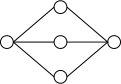
\includegraphics[width=\textwidth]{fig3.pdf}
  \caption{All non-isomorphic graphs with chromatic polynomial $t(t-1)^3(t-2)$.}
  \label{3}
\end{figure}
These are the only three non-isomorphic graphs with chromatic polynomial $t(t-1)^3(t-2)$.

\section{Problem 2}
We can easily see that any graph that contains a vertex with degree $\geq 2$ cannot be a brilliant coloring with $2$ colors as we need $3$. Any graph with $3$ or more vertices (in a connected graph) must contain a vertex with degree at least $2$. Thus, the only colorings of a graph $G$ that is brilliant with $2$ colors are graphs that consist of connected components with $1$ or $2$ vertices. These are forests where each tree has at most $2$ nodes. \\
It is quite easy to see that $P_b(G, t)$ is polynomial in $t$ for every graph $G$ with colors $\{1,..,t\}$. Consider any brilliant coloring of a graph $G$, then by property (1) we have that no two vertices that are adjacent have the same color. This is exactly the requirement for a (non-brilliant) coloring of $G$. This means that any brilliant coloring of $G$ is also just a coloring of $G$. We know that $P(G, t)$ is polynomial in $t$ and since property (2) for a brilliant coloring only restricts what colors we can use, this implies that $P_b(G, t)$ must also be polynomial in $t$.

\section{Problem 3}
Our hypothesis is that
$$
\chi_l(G)+\chi_l(\overline{G})\leq |V(G)|+1
$$
But more specifically, we prove there is a way to color any graph, so that the following holds
\begin{align}\label{eq2}
\chi_l(G)+\chi_l(\overline{G})=|V(G)|+1
\end{align}
which can be extended to show the hypothesis as we do not nessecarily do an optimal coloring.\\
For the induction base, suppose we have a graph $G$ with two vertices that are connected. Obviously, $\chi_l(G)=2$ and $\chi_l(\overline{G})=1$ and so $\chi_l(G)+\chi_l(\overline{G})=3$, which satisfies the hypothesis. In cases $G$ is a graph on two vertices that are not connected, the following proof still works as $G$ and $\overline{G}$ are simply exchanged. \\
\\
For the induction step, we consider adding a new vertex $v$ to $G$. Either this vertex has degree $d_G(v)<\chi_l(G)$ or $d_G(v)\geq \chi_l(G)$. \\
In the first case, when $d_G(v)<\chi_l(G)$, we can use any list of colors of size $\chi_l(G)$ since we would be able to color it with a spare color, so $\chi_l(G)=\chi_l(G+v)$. For the graph $\overline{G}$, we can increase the list chromatic number by one (we might not need to, but for the sake of the proof, we do) and we still have a legal coloring of $\overline{G}$, so $\chi_l(\overline{G}+v)= \chi_l(\overline{G})+1$. Combining the two equations means we have $\chi_l(G+v)+\chi_l(\overline{G}+v)= |V(G+v)|+1$. \\
Conversely, in the second case when $d_G(v)\geq \chi_l(G)$, we see that
\begin{align*}
  d_{\overline{G}}(v)&\leq |V(G)|-\chi_l(G) \\
                     &= \chi_l(\overline{G}))-1 \comment{By rearrangement of Equation \ref{eq2}} \\
                     &< \chi_l(\overline{G})
\end{align*}
Now, just like before, we do not need to increase the list chromatic number in $\overline{G}+v$ as we have a spare color. For $G$, we can again increase the list chromatic number by one and have a legal coloring of $G$. Combining this yields $\chi_l(G+v)+\chi_l(\overline{G}+v)= |V(G+v)|+1$. \\
\\
This means that the following holds everytime we add a vertex $v$:
\begin{align}\label{eq2}
\chi_l(G)+\chi_l(\overline{G})=|V(G)|+1
\end{align}
But since we do not always need to increase the list chromatic number in one of the graphs, we can say it is an upper bound:
$$
\chi_l(G)+\chi_l(\overline{G})\leq |V(G)|+1
$$
This is our hypothesis and what we wanted to prove. However, this proof relies on the idea that adding a vertex cannot increase the list chromatic number by $2$, which I have not been able to prove.

\section{Problem 4}
\subsection{(a)}
We use Sage to estimate $g(n)$. We compute a total of $20$ points, i.e. for the number of vertices $n=\{100,200,..,2000\}$. Sage can generate a random graph $G(n, \frac{1}{2})$, and for each $n$, we perform the greedy coloring of $10$ different graphs in order to find an accurate average. The result from this is seen in Figure \ref{1}, where the $x$-axis is the number of vertices and the $y$-axis is the number of colors used by the greedy coloring algorithm.
\begin{figure}[H]
  \centering
  \captionsetup{justification=centering}
  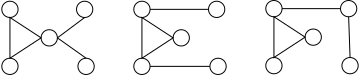
\includegraphics[width=0.8\textwidth]{fig1.pdf}
  \caption{Figure showing how many colors are used by the greedy algorithm as a function of the number of vertices in the graph $G(n, \frac{1}{2})$.}
  \label{1}
\end{figure}
Immediately, we can see a somewhat linear tendency, but this is discussed in the next question. We might be able to be more conclusive if we had run more than $10$ iterations for $n$ to get an even more accurate estimate of $g(n)$.

\subsection{(b)}
If we plot the function $f(n)=\frac{g(n)}{n/\log_2 n}$ as a function of $n$, we get the plot in Figure \ref{2}.
\begin{figure}[H]
  \centering
  \captionsetup{justification=centering}
  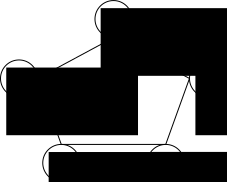
\includegraphics[width=\textwidth]{fig2.pdf}
  \caption{Figure showing the function $f(n)$ as a function of $n$.}
  \label{2}
\end{figure}
It looks like it converges towards $1$ (or rather, vary around $1$), which means we can reasonable suspect that $g(n)$ is asymptotic to $n/\log_2 n$.

\newpage
\subsection{(c)}
A result from Grimmett and McDiarmid\footnote{G. R. Grimmett and C. J. H. McDiarmid, On colouring random graphs, Math. Proc. Cambridge Phil. Soc., 77 (1975), 313--324.} on the chromatic number of random graphs states that:
$$
\frac{n}{2\log_d n} \left(1+o(1)\right)\leq \chi(G_p)\leq \frac{n}{\log_d n}\left(1+o(1)\right)
$$
where $d=1/(1-p)$. Since we got $p=1/2$, we can write:
\begin{align}\label{eq1}
\frac{n}{2\log_2 n} \left(1+o(1)\right)\leq \chi(G_p)\leq \frac{n}{\log_2 n}\left(1+o(1)\right)
\end{align}
So we see the estimation of $g(n)$ we found is the same as the upper bound on the chromatic number from Equation \ref{eq1} (if we disregard the $o(1)$-term). The lower bound on the chromatic number is half the upper bound. This means the greedy algorith  provides results that are at most twice the actual chromatic number, but we can assume that it will probably perform better in most cases (assuming the estimation of $g(n)$ as a fact).

\section{Problem 5}
\subsection{}
I tried to solve 5.1, but have not been able to. My thought was that all the independent sets could correspond to all the ways to use a single color. So instead of having
$$
\sum_I P(G-I, t)
$$
We could assume that one color was accounted for, and instead write something like
$$
t\cdot \sum_I P(G-I, t-1)
$$
But since vertices are removed, this did not really work. I noticed a pattern of alternating sign which makes sense as $P(G, -1)$ yields the number of acyclic orientations, but again I could not find a connection.

\end{document}
